%%%%%%%%%%%%%%%%%%%%%%%%%%%%%%%%%%%%%%%%%%%%%%%%%%%%%%%%%%%%%%%%%%%%%%%%%%%%%%%%
%
% Template license:
% CC BY-NC-SA 3.0 (http://creativecommons.org/licenses/by-nc-sa/3.0/)
%
%%%%%%%%%%%%%%%%%%%%%%%%%%%%%%%%%%%%%%%%%%%%%%%%%%%%%%%%%%%%%%%%%%%%%%%%%%%%%%%%

%----------------------------------------------------------------------------------------
%	PACKAGES AND OTHER DOCUMENT CONFIGURATIONS
%----------------------------------------------------------------------------------------

\documentclass[
11pt, % The default document font size, options: 10pt, 11pt, 12pt
%oneside, % Two side (alternating margins) for binding by default, uncomment to switch to one side
%chapterinoneline,% Have the chapter title next to the number in one single line
spanish,
singlespacing, % Single line spacing, alternatives: onehalfspacing or doublespacing
%draft, % Uncomment to enable draft mode (no pictures, no links, overfull hboxes indicated)
%nolistspacing, % If the document is onehalfspacing or doublespacing, uncomment this to set spacing in lists to single
%liststotoc, % Uncomment to add the list of figures/tables/etc to the table of contents
%toctotoc, % Uncomment to add the main table of contents to the table of contents
parskip, % Uncomment to add space between paragraphs
%codirector, % Uncomment to add a codirector to the title page
headsepline, % Uncomment to get a line under the header
]{MastersDoctoralThesis} % The class file specifying the document structure



%----------------------------------------------------------------------------------------
%	INFORMACIÓN DE LA MEMORIA
%----------------------------------------------------------------------------------------

\thesistitle{Modelos de predicción de \textit{overdue} y
rotación para la redistribución del
crédito financiero} % El títulos de la memoria, se usa en la carátula y se puede usar el cualquier lugar del documento con el comando \ttitle

% Nombre del posgrado, se usa en la carátula y se puede usar el cualquier lugar del documento con el comando \degreename
\posgrado{Carrera de Especialización en Inteligencia Artificial} 
%\posgrado{Carrera de Especialización en Internet de las Cosas} 
%\posgrado{Carrera de Especialización en Intelegencia Artificial}
%\posgrado{Maestría en Sistemas Embebidos} 
%\posgrado{Maestría en Internet de las cosas}

\author{Lic. Paola Mariscal Zegarra} % Tu nombre, se usa en la carátula y se puede usar el cualquier lugar del documento con el comando \authorname

\director{Ing. Yoel Yamil López (FIUBA)} % El nombre del director, se usa en la carátula y se puede usar el cualquier lugar del documento con el comando \dirname
\codirector{Nombre del codirector (pertenencia)} % El nombre del codirector si lo hubiera, se usa en la carátula y se puede usar el cualquier lugar del documento con el comando \codirname.  Para activar este campo se debe descomentar la opción "codirector" en el comando \documentclass, línea 23.

\juradoUNO{Marcos Maillot (pertenencia)} % Nombre y pertenencia del un jurado se usa en la carátula y se puede usar el cualquier lugar del documento con el comando \jur1name
\juradoDOS{Hanes Sciarrone (pertenencia)} % Nombre y pertenencia del un jurado se usa en la carátula y se puede usar el cualquier lugar del documento con el comando \jur2name
\juradoTRES{Pablo Martín Gómez (pertenencia)} % Nombre y pertenencia del un jurado se usa en la carátula y se puede usar el cualquier lugar del documento con el comando \jur3name

\ciudad{Ciudad Autónoma de Buenos Aires}
%\ciudad{ciudad de Mendoza}

\fechaINICIO{abril de 2022}
\fechaFINAL{diciembre de 2022}


\keywords{Sistemas embebidos, FIUBA} % Keywords for your thesis, print it elsewhere with \keywordnames


\begin{document}


\frontmatter % Use roman page numbering style (i, ii, iii, iv...) for the pre-content pages

\pagestyle{plain} % Default to the plain heading style until the thesis style is called for the body content


%----------------------------------------------------------------------------------------
%	RESUMEN - ABSTRACT 
%----------------------------------------------------------------------------------------

\begin{abstract}
\addchaptertocentry{\abstractname} % Add the abstract to the table of contents
%
%The Thesis Abstract is written here (and usually kept to just this page). The page is kept centered vertically so can expand into the blank space above the title too\ldots
\centering

La presente memoria describe el diseño e implementación de un algoritmo predictivo de mora y de rotación del crédito desarrollado para una importante compañía de consumo masivo que otorga créditos a sus clientes para la venta de sus productos. El sistema permite distinguir clientes que por su comportamiento podrían entrar en mora o aquellos que usen en mayor proporción el crédito asignado, lo que permitirá a la compañía mejorar la distribucion del presupuesto destinado a créditos.

Para poder abordar este trabajo se aplicaron conceptos de estadística, bases de datos y aprendizaje automático que permitieron llevar a cabo la implementación de un modelo estadístico basado en machine learning desde la extracción de datos hasta la generación de dos scores: riesgo y rotación

\end{abstract}

%----------------------------------------------------------------------------------------
%	CONTENIDO DE LA MEMORIA  - AGRADECIMIENTOS
%----------------------------------------------------------------------------------------

\begin{acknowledgements}
\addchaptertocentry{\acknowledgementname} % Descomentando esta línea se puede agregar los agradecimientos al índice
\vspace{1.5cm}

A mi familia por apoyarme en cada nuevo desafío.

A mi director, Ing. Yoel Yamil López por su acompañamiento, orientación y por los conocimientos compartidos a lo largo de la carrera.


\end{acknowledgements}

%----------------------------------------------------------------------------------------
%	LISTA DE CONTENIDOS/FIGURAS/TABLAS
%----------------------------------------------------------------------------------------

\tableofcontents % Prints the main table of contents

\listoffigures % Prints the list of figures

\listoftables % Prints the list of tables


%----------------------------------------------------------------------------------------
%	CONTENIDO DE LA MEMORIA  - DEDICATORIA
%----------------------------------------------------------------------------------------

\dedicatory{\textbf{Dedicado a... [OPCIONAL]}}  % escribir acá si se desea una dedicatoria

%----------------------------------------------------------------------------------------
%	CONTENIDO DE LA MEMORIA  - CAPÍTULOS
%----------------------------------------------------------------------------------------

\mainmatter % Begin numeric (1,2,3...) page numbering

\pagestyle{thesis} % Return the page headers back to the "thesis" style

% Incluir los capítulos como archivos separados desde la carpeta Chapters

% Chapter 1

\chapter{Introducción general} % Main chapter title

\label{Chapter1} % For referencing the chapter elsewhere, use \ref{Chapter1} 
\label{IntroGeneral}

%----------------------------------------------------------------------------------------

% Define some commands to keep the formatting separated from the content 
\newcommand{\keyword}[1]{\textbf{#1}}
\newcommand{\tabhead}[1]{\textbf{#1}}
\newcommand{\code}[1]{\texttt{#1}}
\newcommand{\file}[1]{\texttt{\bfseries#1}}
\newcommand{\option}[1]{\texttt{\itshape#1}}
\newcommand{\grados}{$^{\circ}$}

%----------------------------------------------------------------------------------------
%\section{Introducción}
En este capítulo se realiza un acercamiento a los conceptos básicos del aprendizaje automático y financieros. Asimismo, se menciona el estado del arte en un buró de crédito argentino, y por último se explica la motivación, alcance y objetivos del presente trabajo.  
%----------------------------------------------------------------------------------------
\section{Inteligencia artificial en el ámbito financiero}

El sector financiero fué y sigue siendo uno de los pioneros a la hora de implementar inteligencia artificial, una de las tecnologías más revolucionarias de los últimos tiempos.

La inteligencia artificial se refiere a sistemas o máquinas que imitan la inteligencia humana para realizar tareas, mejorando iterativamente a partir de la recopilación de información. Su objetivo es mejorar significativamente las capacidades humanas.
 
Actualmente  la inteligencia artificial mejora el rendimiento y la productividad de las empresas mediante la automatización de los procesos y tareas que antes requerían esfuerzo humano o expertos dedicados a ello.
Hoy en día, muchas aplicaciones de inteligencia artificial son utilizadas tanto por instituciones tradicionales como por \textit{fintech} \cite{molina}. 


El \textit{score} o \textit{scoring} es un método estadístico que predice la probabilidad de \textit{default} o incumplimiento de pago. Se representa con un número que generalmente oscila entre 1 y 999 es el principal factor que analizan los prestamistas ante solicitudes de crédito. Un \textit{score} crediticio que utiliza inteligencia artificial es mucho más completo y sofisticado comparado con criterios tradicionales de \textit{score} de crédito.

En la figura \ref{fig:Figura3}\footnote{Imagen tomada de \url{https://www.bcra.gob.ar/Pdfs/Publicaciones/CreditScoring.pdf}} se observa que  la relación entre el \textit{score} (representado por 'z') y el riesgo no es lineal, por lo que el cambio en el riesgo derivado de un cambio en el \textit{score} depende de los valores que este último tome. Para valores del \textit{score} muy bajos un aumento genera una rápida subida en la probabilidad de cumplimiento y una rápida disminución de la probabilidad de default, mientras que para valores de \textit{score} altos, una mejora hace que la probabilidad de cumplimiento aumente poco y genera una leve caída en el riesgo.

\vspace{1cm}
\begin{figure}[htbp]
	\centering
	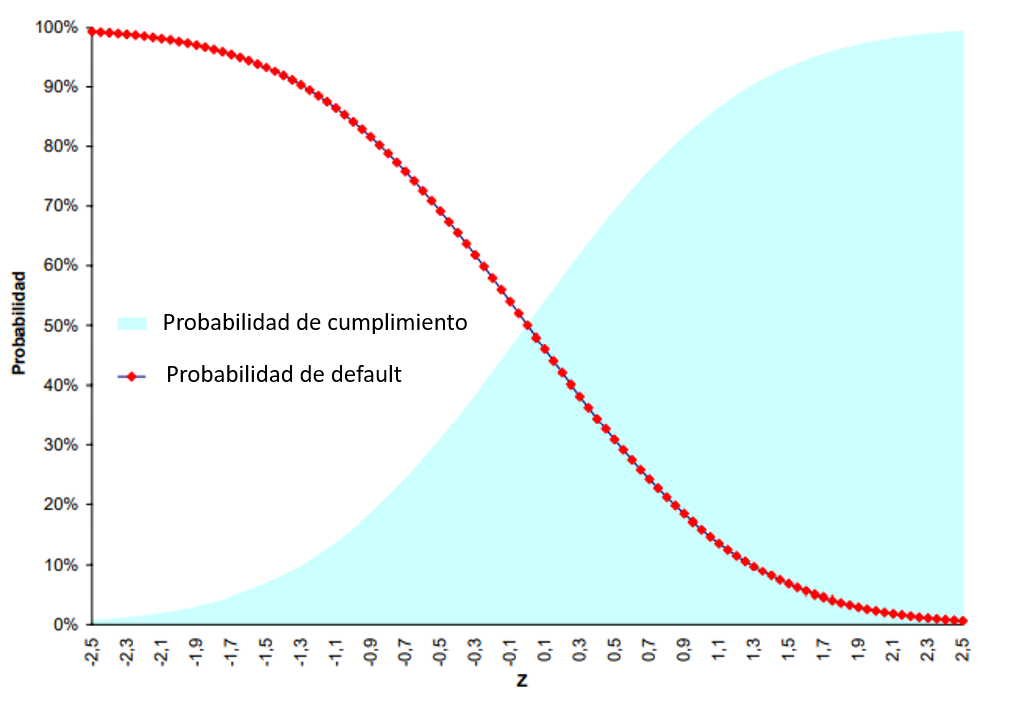
\includegraphics[width=0.8\textwidth]{./Figures/Figura3.png}
	\caption{Relación entre el \textit{score} y el riesgo. 						}
	\label{fig:Figura3}
\end{figure}
\vspace{1cm}

\vspace{1cm}


Los bancos digitales y \textit{fintech} utilizan algoritmos de aprendizaje automático o de máquina cuya importancia radica en la objetividad y la eliminación de sesgos para la toma de decisiones. Asimismo, la capacidad de cómputo de este tipo de sistemas, permite manejar grandes cantidades de datos en poco tiempo y la computación cognitiva ayuda a administrar datos estructurados y no estructurados. Los algoritmos analizan historiales de transacciones e identifican a tiempo signos de futuros problemas.

%\subsection{Una introducción (no tan corta) a \LaTeX{}}

%\subsubsection{Una subsubsección}

%\subsection{Guía matemática rápida para \LaTeX{}}


%----------------------------------------------------------------------------------------

\section{Estado del arte: caso Nosis}

Nosis es una empresa fundada en la década del 80 con el objeto de brindar información de antecedentes comerciales, mercados financieros en línea y comercio exterior para aportar herramientas analíticas que faciliten la toma de decisiones.
Como buró, cuenta con bases de datos exclusivas, información compartida por más de 100 entidades, información pública tanto del BCRA, ANSES, AFIP, entre otros  e innovadoras técnicas analíticas con actualización constante de datos. 

Una de sus principales unidades de negocio trabaja sobre informes comerciales que tienen como variable principal un \textit{score} desarrollado por la misma empresa. 
El \textit{score} de Nosis es un ejemplo de un \textit{score} de riesgo. Brinda información sobre la probabilidad de \textit{default} o mora del cliente consultado desde el momento de la consulta propiamente dicha y 12 meses hacia adelante. Detrás de este número único o calificación, hay más de 70 variables de información dentro del algoritmo desarrollado por la empresa que puso en consideración el endeudamiento histórico de varias fuentes de información y más de 600 atributos de datos. El algoritmo se procesa en el momento de la consulta e indica que cuanto más alto sea el \textit{score}, existe una menor probabilidad de \textit{default} o mora.  
Las bases de datos con las que cuenta Nosis cubren el 99.99\% del endeudamiento de una persona o empresa con el sistema financiero total a nivel país. 

El presente trabajo se centró en el desarrollo de un \textit{score} interno con variables e información de los sistemas transaccionales de la compañía que por un lado permita automatizar el proceso manual llevado a cabo por el área de finanzas, y por el otro, permita evolucionar hacia una estrategia de política crediticia centrada en el comportamiento del cliente con la compañía. 

En la figura \ref{fig:Proceso actual}  se observa el proceso previo al desarrollo del presente trabajo.

\vspace{1cm}
\begin{figure}[htbp]
	\centering
	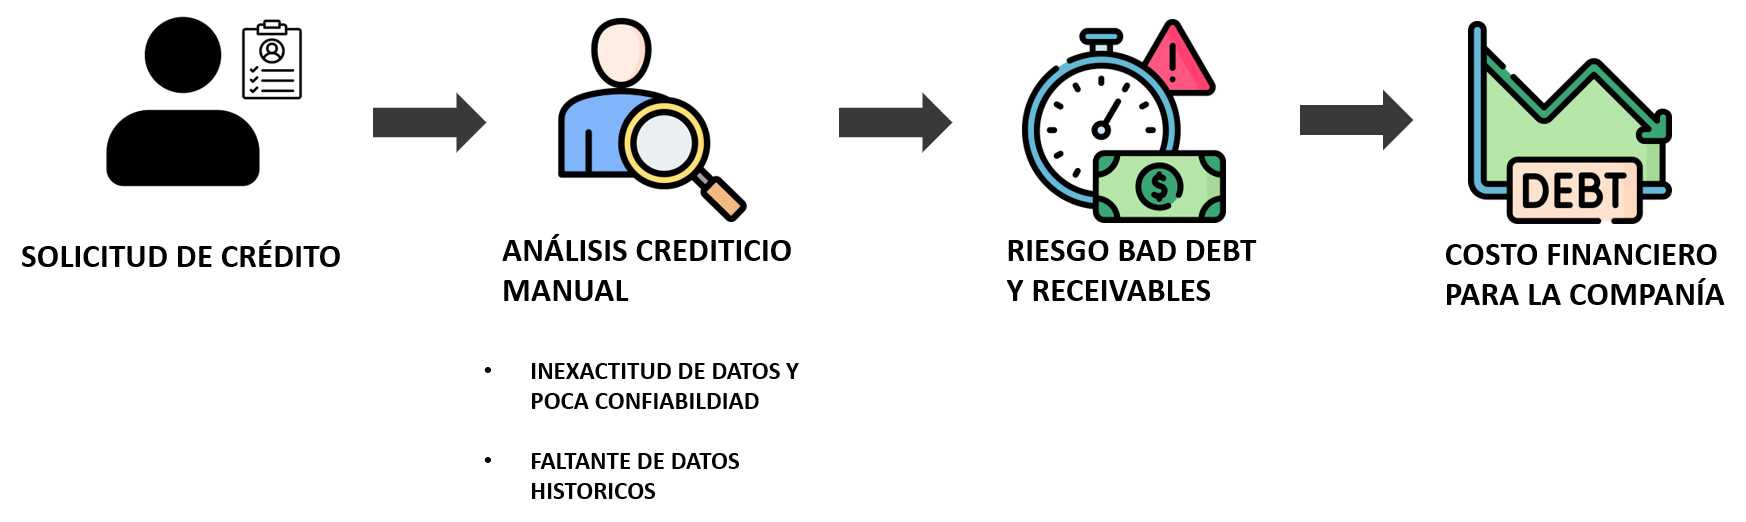
\includegraphics[width=1.0\textwidth]{./Figures/Figura2.png}
	\caption{Proceso previo a la automatización.}
	\label{fig:Proceso actual}
\end{figure}
\vspace{1cm}


%----------------------------------------------------------------------------------------

\section{Motivación}

%\subsection{Carpetas}

La principal motivación para la realización de este trabajo fue la eliminación de subjetividades en procesos de asignación de límite crediticio, la reducción de la deuda generada por los clientes morosos y la optimización del capital empleado (\textit{receivables}) para la generación de mejores resultados, otorgando un mejor servicio de crédito a los clientes, junto a la adopción de tecnologías relacionadas al análisis predictivo en una empresa tradicional de muchos años y con procesos establecidos adversos al cambio.

La no existencia de una herramienta que permita objetivamente asignar límite de crédito a cada cliente significaba un alto riesgo asociado a la mora o incobrabilidad. De hecho, durante el año 2021 el \textit{bad debt} o deuda incobrable ascendía casi al 30\% de la cartera de clientes con crédito. Por otro lado, la compañía no estaba cobrando interés alguno por los créditos cedidos y el P\&L de crédito (\textit{profit and loss}) arrojaba resultados negativos por un porcentaje considerable de clientes en mora sin un ROIC (\textit{return on invested capital})asociado.

En referencia a la opinión de los clientes en temáticas de crédito, se obtuvo un bajo NPS (\textit{net promoter score}) en las encuestas de satisfacción de servicio enviadas.
Sumado a lo anteriormente mencionado se encontraban a menudo errores manuales en análisis o asignación de crédito  por causa de la no automatización de procesos. Existía la dependencia de personal específico solo para realizar un análisis de riesgo de cada cliente a partir de reglas de negocio definidas.

El presente trabajo fue el primer algoritmo desarrollado por el área de \textit{data analytics} y el principal caso de uso dentro de la compañía, rompiendo así la brecha entre las áreas de negocio y de TI (tecnología de la información).


%----------------------------------------------------------------------------------------

\section{Objetivos y alcance}

\subsection{Objetivos}

El propósito de este trabajo consistió esencialmente en el diseño, pruebas e implementación de una solución de inteligencia artificial que permite estimar la mora
y la rotación del crédito de los clientes activos de la compañía, asegurando a una mejor distribución de los recursos crediticios, considerando distintos aspectos del cliente en cuanto a compras, pagos atrasados, deuda total vigente, cheques rechazados, antigüedad e historial de pagos, entre otras variables.

En la figura \ref{fig:Diagrama en bloques del sistema}  se observa un diagrama general de la solución y las etapas que la componen.

\vspace{1cm}
\begin{figure}[htbp]
	\centering
	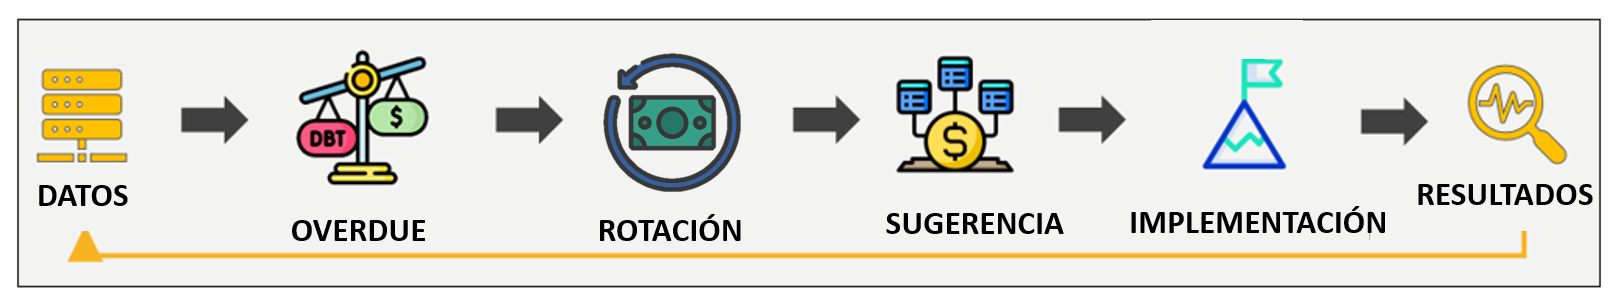
\includegraphics[width=1.0\textwidth]{./Figures/Diagrama de FlujoV2.png}
	\caption{Diagrama en bloques del sistema.}
	\label{fig:Diagrama en bloques del sistema}
\end{figure}
\vspace{1cm}

\vspace{1cm}

En el capítulo \ref{Chapter3} se detalla el diseño y la implementación de las etapas que componen este sistema.

	
\subsection{Alcance}


El alcance de este trabajo estuvo orientado a desarrollar una solución de software que permite cubrir aspectos que giran en torno a los siguientes ejes:

\begin {enumerate}
\item Entendimiento del problema: 
	\begin {itemize}
	\item \textit{Assesment} del proceso de asignación manual del límite de
crédito. 
	\item Resultados esperados a partir de la implementación de la solución.
	\end {itemize}

	
\item Aspectos relacionados al entendimiento del negocio: 
	\begin {itemize}
	\item Entendimiento de las restricciones asociadas al proceso. 
	\item Entendimiento de aspectos generales del negocio.
	\end {itemize}
	
\item Aspectos relacionados a la adquisición y comprensión de datos: 
	\begin {itemize}
	\item \textit{Assesment} de las fuentes de datos (modelos en \textit{datawarehouse} y otras). 
	\item Exploración de los datos para determinar la calidad de la información.
	\end {itemize}
	
\item Aspectos relacionados al modelado: 
	\begin {itemize}
	\item Diseño de características: generación de variables adicionales a partir de los datos sin procesar para facilitar 
el entrenamiento del modelo.
	\item Entrenamiento del modelo: elección del modelo que responda a la pregunta de negocio con la máxima precisión, evaluando métricas de éxito.
	\end {itemize}
	
\item Aspectos relacionados al despliegue: 
	\begin {itemize}
	\item Implementación del/los modelo/s en un entorno de producción o similar para el consumo por el usuario final o aplicaciones. 
	\end {itemize}
\end {enumerate}
 
El alcance de este trabajo no cubre:
\begin {itemize}
\item El mantenimiento de la base de datos en la cual se aloja la información generadora de la entrada para el modelo de inteligencia artificial.
\item La instalación y mantenimiento del \textit{hardware} necesario para el procesamiento de información del modelo desarrollado.
\item La disponibilización de la salida del algoritmo directamente en alguna aplicación de la compañía.
\end {itemize}
\chapter{Introducción específica} % Main chapter title

\label{Chapter2}

%----------------------------------------------------------------------------------------
%	SECTION 1
%----------------------------------------------------------------------------------------
En este capítulo se detallan los requerimientos asociados al desarrollo y la implementación de los modelos, así como el contexto y las necesidades de negocio. Finalmente se especificarán las tecnologías aplicadas en el desarrollo del trabajo,
destacando los componentes de inteligencia artificial seleccionados para la predicción de la mora y la rotación. 

\section{Requerimientos asociados al desarrollo e implementación de/los modelo/s}
\label{sec:ejemplo}

\subsection{Requerimientos asociados al desarrollo}

\begin{enumerate}

\item Los códigos deben desarrollarse con herramientas de Microsoft Azure que es el servicio de computación en la nube utilizado por el área de data \textit{analytics}.
\item El equipo de desarrollo tiene la potestad de utilizar el lenguaje de su conocimiento para el desarrollo del código del modelo.
\item Se utiliza GIT como repositorio para el control de versionado de código.


\end{enumerate}


\subsection{Requerimientos asociados a la implementación}
\label{subsec:ejemplo}

\begin{enumerate}
\item Se utiliza Azure Databricks como herramienta tanto para el entrenamiento de los modelos como para su implementación.
\item Debe existir un archivo de ejecución principal llamado \textit{main.py} y un \textit{job} de ejecución automática de ese archivo en Databricks para la implementación \textit{batch}, es decir sin supervisión.
\item Utilización de MLflow, una plataforma de código abierto para la administración del ciclo de vida de los modelos de aprendizaje automático, para el despliegue en producción y el seguimiento de los desarrollos dentro de la compañía.
\end{enumerate}


\section{Modelos de inteligencia artificial utilizados}\label{sec:Modelos}

Como se desarrollará en los próximos capitulos, el modelo elegido para el planteo de la solución fue la regresión logística.
La regresión logística es un modelo de clasificación, también conocida como regresión logit o clasificador de máxima entropía y se encuadra dentro de los modelos lineales generalizados.
La regresión logística describe la probabilidad de que la variable objetivo pertenezca a una clase o a otra: dado un cierto valor límite, si el valor de la variable objetivo iguala o excede dicho valor, se devuelve como predicción la clase "positiva", caso contrario se devuelve como predicción la clase "negativa". Para ello se utiliza la función logística o también llamada función sigmoide, que siempre devuelve un valor entre 0 y 1. A continuación se detalla la función:

\begin{center}
\begin{LARGE}
función sigmoide = $f(x)$ = $\frac{1}{1+e^{-x}}$

\end{LARGE}
\end{center}

En la figura \ref{fig:funcionlog} se puede observar la curva logística:

\vspace{1cm}
\begin{figure}[htbp]
	\centering
	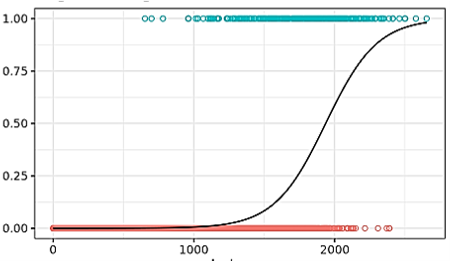
\includegraphics[width=0.8\textwidth]{./Figures/funcionlog.png}
	\caption{Gráfico función logística}
	\label{fig:funcionlog}
\end{figure}
\vspace{1cm}

\vspace{1cm}

La variable ''Y'' a predecir es cualitativa debido a que el objetivo es predecir la probabilidad que un sujeto tome una determinada decisión de índole discreta, condicionada a ciertas variables explicativas y permitiendo identificar las características del sujeto con variables independientes cualitativas.


Para valores de x muy grandes positivos, el valor de $e^{-x}$ es aproximadamente 0 por lo que el valor de la función sigmoide es 1. Para valores de x muy grandes negativos, el valor de $e^{-x}$ tiende a infinito por lo que el valor de la función sigmoide es 0. 

Un punto importante a tener en cuenta a la hora de implementar este modelo es que el set de datos con los que se trabaje debe ser normalizado porque de lo contrario podrían encontrarse indeterminaciones matemáticas.

\section{Herramientas de software utilizadas}
\subsection{Espacio de trabajo: Databricks}
Databricks es una plataforma que facilita la creación y ejecución de \textit{pipelines} o canales de datos permitiendo la colaboración en proyectos de ciencia de datos y analíticos para la construcción e implementación de modelos de aprendizaje de máquina.
Al mismo tiempo, ofrece soluciones de ingeniería de datos, administración, seguridad, gobernanza, entre otros. Está basado en código y estándares abiertos para maximizar su flexibilidad. El enfoque unificado simplifica la arquitectura de datos al eliminar los silos de datos que tradicionalmente separan la analítica, la inteligencia de negocios, la ciencia de datos y el aprendizaje automático.
En la figura  \ref{fig:databricks} se puede visualizar la arquitectura de Databricks:

\vspace{1cm}
\begin{figure}[htbp]
	\centering
	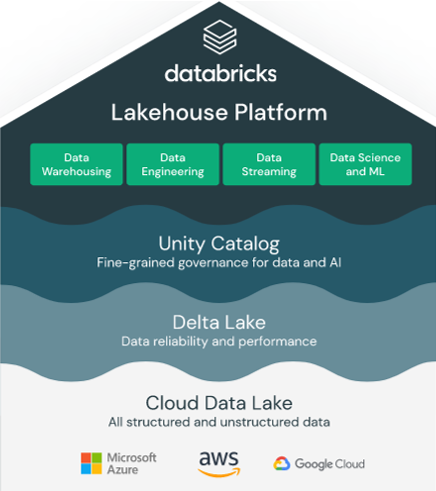
\includegraphics[width=0.7\textwidth]{./Figures/databricks.png}
	\caption{Arquitectura general de la plataforma Databricks.}
	\label{fig:databricks}
\end{figure}
\vspace{1cm}


En cuanto a la terminología utilizada dentro de la plataforma, se pueden detallar los siguientes conceptos clave:

\begin{itemize}
\item Espacio de trabajo: permiten organizar todo el trabajo realizado dentro de la plataforma similar a una estructura de carpetas que permite guardar archivos, bibliotecas utilizadas para la operación y manipulación de datos e incluso compartirlas con otros usuarios.
\item \textit{Notebooks}: se podría definir como conjunto de celdas que permiten ejecutar determinados comandos. Soporta cualquier tipo de lenguaje de programación como Scala, Python, R, SQL, entre otros. Los \textit{notebook} deben estar conectados a un cluster para ejecutar comandos. Se pueden compartir o descargar de forma local.
\item Librerías: son paquetes o módulos que proporcionan una funcionalidad adicional para la resolución de problemas de negocio. Facilitan la programación al proporcionar funcionalidades comunes, que han sido resueltas previamente por otros programadores.
\item Tablas: son datos estructurados utilizados para el análisis, representados por una colección de filas y columnas almacenados como archivos de datos en el almacenamiento de objetos o base de datos.
\item \textit{Clusters}: son grupos de ordenadores que se tratan como un único ordenador. Permiten ejecutar \textit{notebooks} o bibliotecas sobre un conjunto de datos. Cada clúster tiene controles de acceso para garantizar la seguridad de la información 
\item \textit{Jobs}: Los \textit{jobs} son la herramienta mediante la cual se puede programar la ejecución para que se produzca en un clúster ya existente o en un clúster propio. 
\item Aplicaciones: son integraciones de terceros con la plataforma Databricks.Entre ellas se encuentran aplicaciones como Power BI
\end{itemize}
 
\subsection{Motor de análisis y procesamiento: Spark}
Es un motor de análisis unificado para el procesamiento de datos a gran escala. Proporciona una interfaz de programación de aplicaciones de alto nivel, conocida también por la sigla API que es un conjunto de subrutinas, funciones y procedimientos que ofrece la biblioteca para ser utilizada por otro software como capa de abstracción. 
Es compatible con Spark SQL para consultas y procesamiento de datos en SQL, MLlib para el aprendizaje automático o GraphX para procesamiento de gráficos.
Como se menciona en la sección \ref{sec:Modelos}, para el presente trabajo se utilizó la regresión logística como método para predecir la mora y la rotación de un cliente. A continuación se muestra mediante un ejemplo, cómo cargar un conjunto de datos de muestra, construir un modelo de regresión logística y hacer predicciones con el modelo resultante para calcular el error de entrenamiento:

\begin{lstlisting}
from pyspark.mllib.classification import LogisticRegressionWithLBFGS, LogisticRegressionModel
from pyspark.mllib.regression import LabeledPoint

# Load and parse the data 
def parsePoint(line):
    values = [float(x) for x in line.split(' ')]
    return LabeledPoint(values[0], values[1:])

data = sc.textFile("data/mllib/sample_svm_data.txt")
parsedData = data.map(parsePoint)

# Build the model
model = LogisticRegressionWithLBFGS.train(parsedData)

# Evaluating the model on training data
labelsAndPreds = parsedData.map(lambda p: (p.label, model.predict(p.features)))
trainErr = labelsAndPreds.filter(lambda lp: lp[0] != lp[1]).count() / float(parsedData.count())
print("Training Error = " + str(trainErr))

# Save and load model
model.save(sc, "target/tmp/pythonLogisticRegression")
sameModel = LogisticRegressionModel.load(sc,
                                         "target/tmp pythonLogisticRegression")
\end{lstlisting}

\subsection{Lenguaje de programación: Python}
\textit{Python} es un lenguaje de programación que permite trabajar rápidamente e integrar sistemas de forma más eficaz. Entre sus ventajas de uso se puede enumerar:
\begin{enumerate}
\item Amigable y fácil de aprender: existe una comunidad que organiza conferencias y reuniones para facilitar la colaboración entre los programadores. Cuenta con una extensa y detallada documentación que incluye especificaciones de versiones, tutoriales, librerías, módulos, reporte de errores, entre otros.
\item Variedad de aplicaciones: el índice de paquetes de \textit{Python} (PyPI) alberga miles de módulos de terceros para \textit{Python}. Tanto la biblioteca estándar de \textit{Python} como los módulos aportados por la comunidad permiten un sinfín de posibilidades.
\item Código abierto: \textit{Python} está desarrollado bajo una licencia de código abierto aprobada por la OSI (\textit{Open Source Initiative}), lo que hace que se pueda utilizar y distribuir libremente, incluso para uso comercial. La licencia de \textit{Python} es administrada por la \textit{Python Software Foundation}.
\end{enumerate}


\subsection{Gestión del código y versiones: GitHub}
GitHub es una plataforma de alojamiento de código para el control de versiones y la colaboración.Permite trabajar de forma colaborativa en proyectos desde cualquier lugar. A continuación, se enumeran los conceptos escenciales referidos a la plataforma:

\begin{itemize}
\item Repositorios: un repositorio contiene todos los archivos de un proyecto y el historial de revisiones de cada archivo. Existe la posibilidad de discutir y gestionar el trabajo del proyecto dentro del repositorio.
\item Ramas: una rama es una versión paralela de un repositorio. Está contenida dentro del repositorio, pero no afecta a la rama primaria o principal, lo que le permite trabajar libremente sin interrumpir la versión "viva". Cuando se hayan realizado cambios, se puede  fusionar dicha rama de nuevo con la rama principal para publicar los cambios o dicho de otra manera, realizar un \textit{pull request}.
\item \textit{Commits}: un commit, o "revisión", es un cambio individual en un archivo (o conjunto de archivos). Cuando se hace un commit para guardar el trabajo realizado, Git crea un ID único (también conocido como "SHA" o "\textit{hash}") que permite mantener un registro de los cambios específicos confirmados junto con quién los hizo y cuándo. Los \textit{commits} suelen contener un mensaje de \textit{commit} que es una breve descripción de los cambios realizados.
\item Pull requests: las solicitudes de incorporación de cambios permiten comunicar acerca de los cambios insertados en una rama de un repositorio en GitHub. Una vez que se abre una solicitud de incorporación de cambios, se puede debatir y revisar los posibles cambios con los colaboradores y agregar confirmaciones de seguimiento antes de que los cambios se fusionen en la rama base.
\end{itemize}

\subsection{Creación del proyecto, seguimiento y registro del modelo: MLFlow}
MLFlow es una plataforma de código abierto para el ciclo de vida del aprendizaje automático incluyendo la experimentación, la reproducibilidad, el despliegue y un registro central de modelos. Trabaja perfectamente integrado con Python, Apache Spark, Azure Machine Learning, Databricks, entre otros.
Aborda cuatro funciones principales:
\begin{enumerate}
\item MLflow Tracking: seguimiento de experimentos para registrar y comparar parámetros y resultados.
\item MLflow Projects: empaquetado del código de forma reutilizable y reproducible para compartirlo con otros científicos de datos o transferirlo a producción. 
\item MLflow Models: gestión y despliegue de modelos desde una variedad de bibliotecas de aprendizaje automático a una variedad de plataformas de inferencia y servicio de modelos. 
\item MLflow Model Registry: proporciona un almacén central de modelos para gestionar de forma colaborativa el ciclo de vida completo de un modelo MLflow, incluyendo el versionado de modelos, las transiciones de etapas y las anotaciones.
MLflow es agnóstico a las librerías. Se puede utilizar con cualquier biblioteca de aprendizaje automático, y en cualquier lenguaje de programación, ya que todas las funciones son accesibles a través de una API REST y CLI.
\end{enumerate}

\subsection{Programación de flujos: Apache Airflow}
Airflow es una plataforma creada por la comunidad para crear, programar y supervisar flujos de trabajo de forma programada. Se basa en las siguientes características:
\begin{itemize}
\item \textit{Python} puro: con conocimientos básicos de Python, es posible es posible crear flujos de trabajo propios, incluyendo los formatos de fecha y hora para la programación y los bucles para generar dinámicamente las tareas. Esto permite mantener una flexibilidad total al construir flujos de trabajo.
\item Interfaz de usuario útil: es posible gestionar, supervisar y programar los flujos de trabajo a través de una aplicación web sólida y moderna, contando con una visión completa del estado y los registros de las tareas completadas y en curso.
\item Integraciones robustas: proporciona muchos operadores \textit{plug-and-play} que están listos para ejecutar sus tareas en Google Cloud Platform, Amazon Web Services, Microsoft Azure y muchos otros servicios de terceros. Esto hace que \textit{Airflow} sea fácil de aplicar a la infraestructura actual y de ampliar a las tecnologías de próxima generación.
\item Fácil de usar: cualquier persona con conocimientos de Python puede desplegar un flujo de trabajo. \textit{Apache Airflow} no limita el alcance de \textit{pipelines}; se puede utilizar para construir modelos de ML, transferir datos, gestionar infraestructura, entre otros.
\item Código abierto: donde se desee compartir una mejora o cambio, se puede hacer abriendo un \textit{pull request}. Sencillo, sin barreras ni procedimientos prolongados.
\end{itemize} 
\chapter{Diseño e implementación} % Main chapter title

\label{Chapter3} % Change X to a consecutive number; for referencing this chapter elsewhere, use \ref{ChapterX}

\definecolor{mygreen}{rgb}{0,0.6,0}
\definecolor{mygray}{rgb}{0.5,0.5,0.5}
\definecolor{mymauve}{rgb}{0.58,0,0.82}

%%%%%%%%%%%%%%%%%%%%%%%%%%%%%%%%%%%%%%%%%%%%%%%%%%%%%%%%%%%%%%%%%%%%%%%%%%%%%
% parámetros para configurar el formato del código en los entornos lstlisting
%%%%%%%%%%%%%%%%%%%%%%%%%%%%%%%%%%%%%%%%%%%%%%%%%%%%%%%%%%%%%%%%%%%%%%%%%%%%%
\lstset{ %
  backgroundcolor=\color{white},   % choose the background color; you must add \usepackage{color} or \usepackage{xcolor}
  basicstyle=\footnotesize,        % the size of the fonts that are used for the code
  breakatwhitespace=false,         % sets if automatic breaks should only happen at whitespace
  breaklines=true,                 % sets automatic line breaking
  captionpos=b,                    % sets the caption-position to bottom
  commentstyle=\color{mygreen},    % comment style
  deletekeywords={...},            % if you want to delete keywords from the given language
  %escapeinside={\%*}{*)},          % if you want to add LaTeX within your code
  %extendedchars=true,              % lets you use non-ASCII characters; for 8-bits encodings only, does not work with UTF-8
  %frame=single,	                % adds a frame around the code
  keepspaces=true,                 % keeps spaces in text, useful for keeping indentation of code (possibly needs columns=flexible)
  keywordstyle=\color{blue},       % keyword style
  language=[ANSI]C,                % the language of the code
  %otherkeywords={*,...},           % if you want to add more keywords to the set
  numbers=left,                    % where to put the line-numbers; possible values are (none, left, right)
  numbersep=5pt,                   % how far the line-numbers are from the code
  numberstyle=\tiny\color{mygray}, % the style that is used for the line-numbers
  rulecolor=\color{black},         % if not set, the frame-color may be changed on line-breaks within not-black text (e.g. comments (green here))
  showspaces=false,                % show spaces everywhere adding particular underscores; it overrides 'showstringspaces'
  showstringspaces=false,          % underline spaces within strings only
  showtabs=false,                  % show tabs within strings adding particular underscores
  stepnumber=1,                    % the step between two line-numbers. If it's 1, each line will be numbered
  stringstyle=\color{mymauve},     % string literal style
  tabsize=2,	                   % sets default tabsize to 2 spaces
  title=\lstname,                  % show the filename of files included with \lstinputlisting; also try caption instead of title
  morecomment=[s]{/*}{*/}
}


%----------------------------------------------------------------------------------------
%	SECTION 1
%----------------------------------------------------------------------------------------
\section{Arquitectura del sistema completo}
\vspace{1cm}
\begin{figure}[htbp]
	\centering
	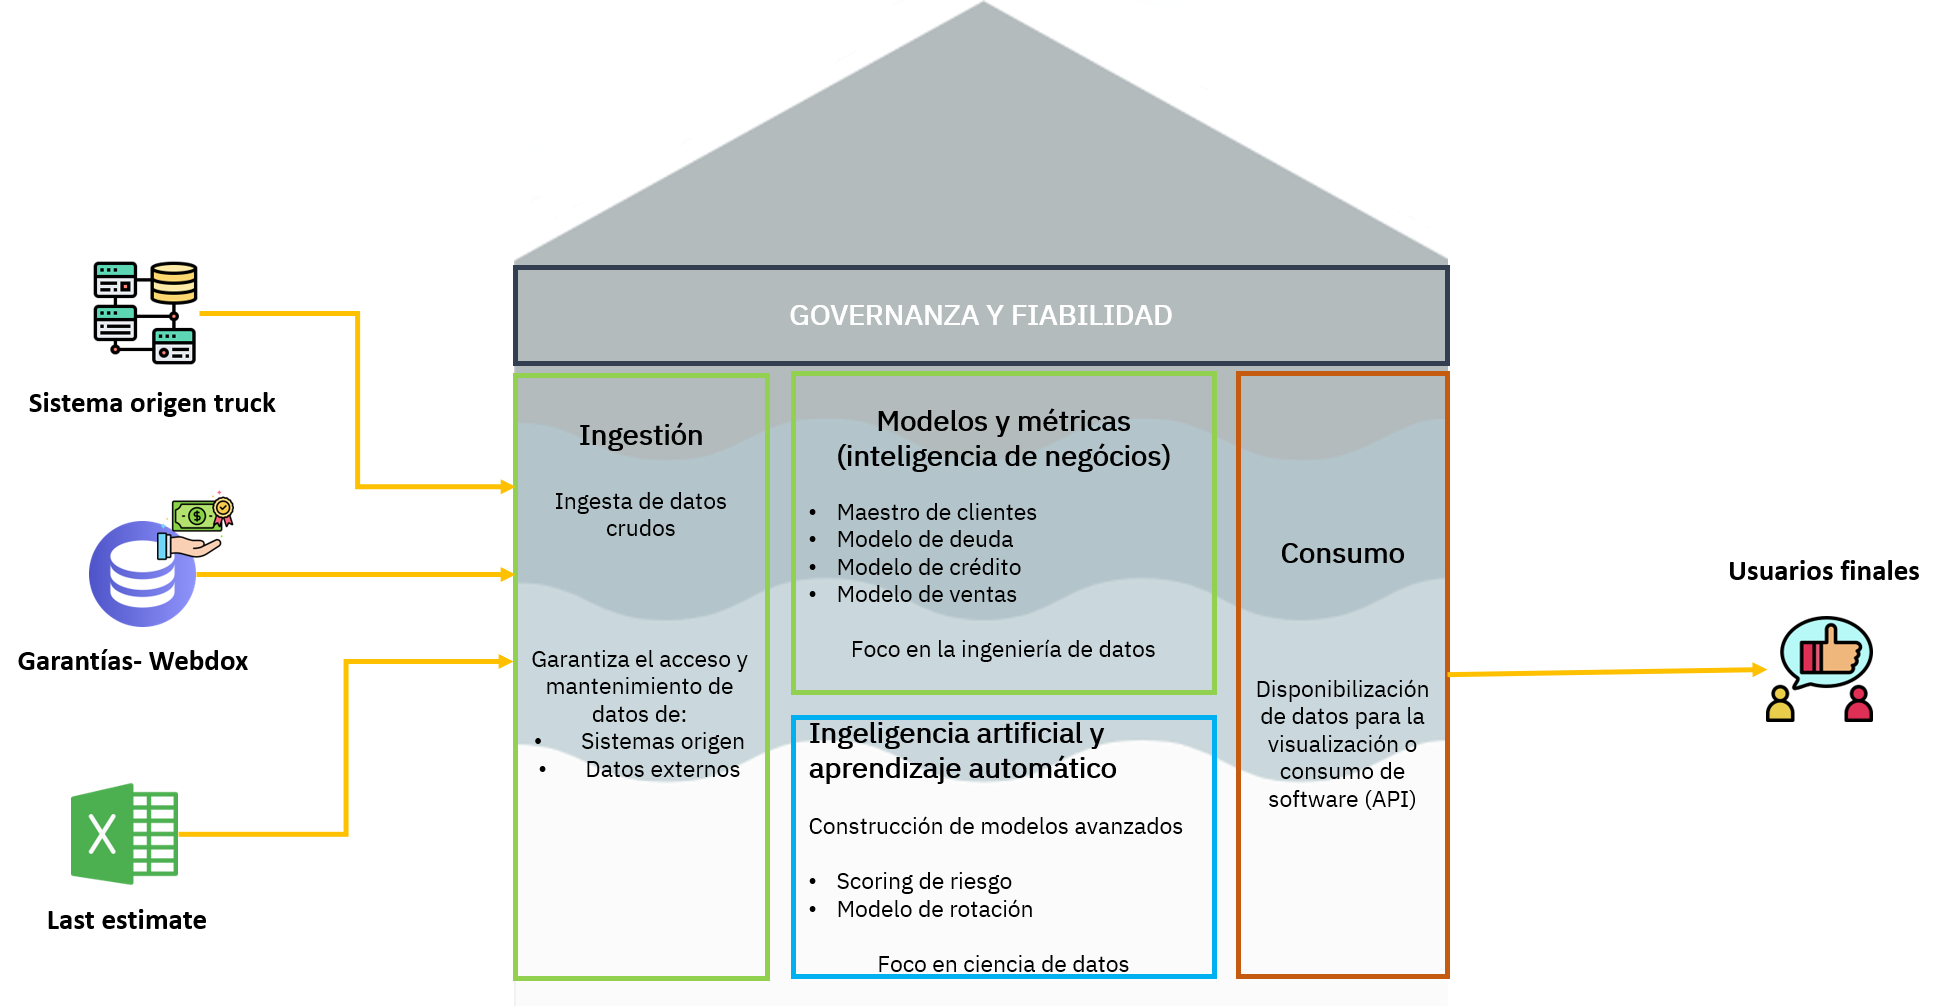
\includegraphics[width=1.0\textwidth]{./Figures/arqcompleta.png}
	\caption{Arquitectura completa.}
	\label{fig:arqcompleta}
\end{figure}
\vspace{1cm}




\section{Generación y tratamiento de los datos}
\section{Automatización e implementación}




% Chapter Template

\chapter{Ensayos y resultados} % Main chapter title

\label{Chapter4} % Change X to a consecutive number; for referencing this chapter elsewhere, use \ref{ChapterX}

%----------------------------------------------------------------------------------------
%	SECTION 1
%----------------------------------------------------------------------------------------

\section{Descripción del banco de pruebas}
\label{sec:pruebasHW}

\section{Modelos probados}
\section{Descripción de la salida}
\section{Caso de uso}

 
% Chapter Template

\chapter{Conclusiones} % Main chapter title

\label{Chapter5} % Change X to a consecutive number; for referencing this chapter elsewhere, use \ref{ChapterX}


%----------------------------------------------------------------------------------------

%----------------------------------------------------------------------------------------
%	SECTION 1
%----------------------------------------------------------------------------------------

\section{Conclusiones generales}



%----------------------------------------------------------------------------------------
%	SECTION 2
%----------------------------------------------------------------------------------------
\section{Trabajo futuro} 

%----------------------------------------------------------------------------------------
%	CONTENIDO DE LA MEMORIA  - APÉNDICES
%----------------------------------------------------------------------------------------

\appendix % indicativo para indicarle a LaTeX los siguientes "capítulos" son apéndices

% Incluir los apéndices de la memoria como archivos separadas desde la carpeta Appendices
% Descomentar las líneas a medida que se escriben los apéndices

%% Appendix A

\chapter{Appendix Title Here} % Main appendix title

\label{AppendixA} % For referencing this appendix elsewhere, use \ref{AppendixA}

Write your Appendix content here.
%\include{Appendices/AppendixB}
%\include{Appendices/AppendixC}

%----------------------------------------------------------------------------------------
%	BIBLIOGRAPHY
%----------------------------------------------------------------------------------------

\Urlmuskip=0mu plus 1mu\relax
\raggedright
\printbibliography[heading=bibintoc]

%----------------------------------------------------------------------------------------

\end{document}  
